\documentclass[../../course]{subfiles}

\renewcommand\thesection{\arabic{section}}


\begin{document}

\section{Generating Sequences} \label{sec:wrkGenSeqs}

First of all we need to generate these three sequences, with frequences of:

\begin{align}
    f_{1} &= 28 \si{Hz}                     \label{eqn:freq1} \\
    f_{2} &= 28 + 0.1      = 28.1   \si{Hz} \label{eqn:freq2} \\
    f_{3} &= (2 \times 28) = 56     \si{Hz} \label{eqn:freq3}
\end{align}

Now we need to decide whether we need to generate a \emph{sine} signal or one with
$90 \degree$ phase shift, ie, the \emph{cosine} signal. If we mix\footnote{like, real
part and imaginary part having a phase difference} \emph{sine} and \emph{cosine} we may
get a different kind of \emph{complex} sequence than if we mix \emph{sine} to \emph{sine}
or \emph{cosine} to \emph{cosine}. For our analysis, let's stick with having zero phase
shift between the signals that we are mixing. So let's just mix \emph{sine} signals with
the above frequencies.


To get the continous feel of these sequences let's generate them with $2500$ samples.
And these signals will range from $0$ to $\frac{\pi}{4}$.


Therefore these signals will be:

\begin{align}
    x_{1}(t) =
    \begin{cases}
        \sin(2 \pi 28 t) & \text{; for} \; 0 \le t \le \dfrac{\pi}{4}
    \end{cases}
    \label{eqn:seqx1}
\end{align}

\begin{align}
    x_{2}(t) =
    \begin{cases}
        \sin(2 \pi 28.1 t) & \text{; for} \; 0 \le t \le \dfrac{\pi}{4}
    \end{cases}
    \label{eqn:seqx2}
\end{align}

\begin{align}
    x_{3}(t) =
    \begin{cases}
        \sin(2 \pi 56 t) & \text{; for} \; 0 \le t \le \dfrac{\pi}{4}
    \end{cases}
    \label{eqn:seqx3}
\end{align}

\subsection{Python Implementation} \label{lst:threeSeqs}

%python/three_sequences.py%
\begin{minted}[breaklines, autogobble, mathescape] {python}
    import numpy as np
    import pandas as pd

    F = 28
    t = np.linspace(0, 1.25 * np.pi / 4, 2500)

    x1 = np.sin( 2 * np.pi * F * t)
    x2 = np.sin( 2 * np.pi * (F + 0.1) * t)
    x3 = np.sin( 2 * np.pi * 2 * F * t)

    data = pd.DataFrame(
        {
            "x1": x1,
            "x2": x2,
            "x3": x3,
        }
    )

    data.to_csv(
        "../data/three_sequences.csv", sep = " ", index_label = "time"
    )
    print(data)

\end{minted}

\paragraph{Output}

\begin{minted}[breaklines, autogobble] {text}
                x1        x2        x3
    0     0.000000  0.000000  0.000000
    1     0.069060  0.069306  0.137790
    2     0.137790  0.138279  0.272951
    3     0.205862  0.206587  0.402906
    4     0.272951  0.273901  0.525174
    ...        ...       ...       ...
    2495  0.339117 -0.266620 -0.638045
    2496  0.273340 -0.332776 -0.525861
    2497  0.206258 -0.397332 -0.403645
    2498  0.138190 -0.459977 -0.273729
    2499  0.069463 -0.520410 -0.138590

    [2500 rows x 3 columns]
\end{minted}

\subsubsection{Plots}

\begin{figure} [H]
    \centering
    \adjustbox{max width = \textwidth} {
        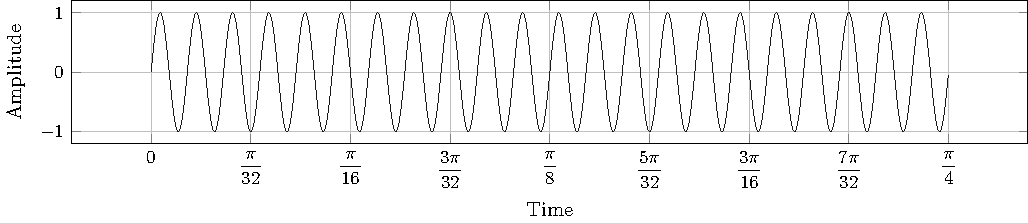
\includegraphics[height = 0.8\textheight] {tikzpics/plotSeqX1.pdf}
    }
    \captionof{figure} {Sine signal $x_{1}$ with frequency of $28 \si{Hz}$}
    \label{plt:seqx1}
\end{figure}

\begin{figure} [H]
    \centering
    \adjustbox{max width = \textwidth} {
        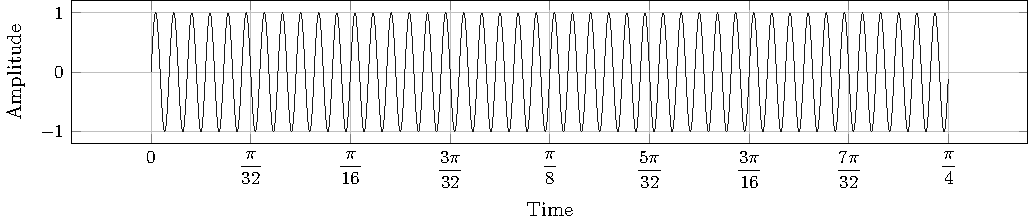
\includegraphics[height = 0.8\textheight] {tikzpics/plotSeqX2.pdf}
    }
    \captionof{figure} {Sine signal $x_{2}$ with frequency of $28.1 \si{Hz}$}
    \label{plt:seqx2}
\end{figure}

\begin{figure} [H]
    \centering
    \adjustbox{max width = \textwidth} {
        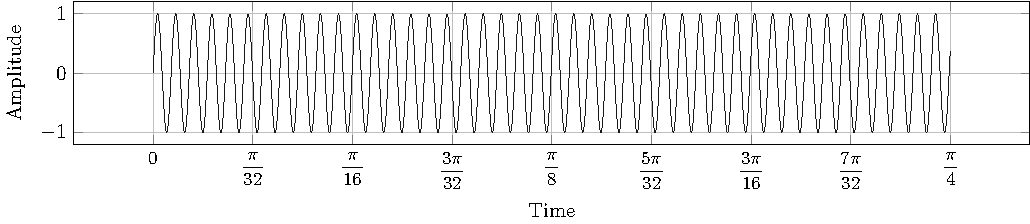
\includegraphics[height = 0.8\textheight] {tikzpics/plotSeqX3.pdf}
    }
    \captionof{figure} {Sine signal $x_{3}$ with frequency of $56 \si{Hz}$}
    \label{plt:seqx3}
\end{figure}

\end{document}
